\subsection{Risultati per linea}
\label{sec:risultati-linee}
Gli indicatori complessivi nascondono differenze forti fra le linee. La \cref{tab:linee-ritardi} riporta, per ognuna delle 61 linee nel giorno feriale, le corse, i treni utilizzati con il loro tipo, la puntualità a destinazione e il ritardo medio nell'orario reale e nei due scenari del Passante. I treni sono quelli assegnati dal modello con la regola descritta nella \cref{sec:orari}, e il tipo deriva dalla ripartizione per linea.

{\small
\begin{longtable}{@{}lrr>{\raggedright\arraybackslash}p{0.36\textwidth}rrrr@{}}
	\caption{Giorno feriale: corse, treni utilizzati e ritardo medio per linea. La puntualità è quella a destinazione nell'orario reale; il ritardo medio è in secondi.}\label{tab:linee-ritardi}\\
	\toprule
	 & & & & & \multicolumn{3}{c}{Ritardo medio (s)} \\
	Linea & Corse & Treni & Tipi di treno & Punt. & Reale & 15 min & 10 min \\
	\midrule
	\endfirsthead
	\toprule
	 & & & & & \multicolumn{3}{c}{Ritardo medio (s)} \\
	Linea & Corse & Treni & Tipi di treno & Punt. & Reale & 15 min & 10 min \\
	\midrule
	\endhead
	S1 & 74 & 7 & 4 TSR, 1 Caravaggio 5, 1 ETR 245, 1 TAF & 100\% & 16 & 16 & 16 \\
	S2 & 62 & 5 & 3 TSR, 1 Caravaggio 5, 1 ETR 245 & 100\% & 11 & 11 & 49 \\
	S3 & 76 & 4 & 3 Caravaggio 5, 1 TSR & 100\% & 17 & 17 & 17 \\
	S4 & 73 & 6 & 4 Caravaggio 5, 2 TSR & 100\% & 28 & 39 & 50 \\
	S5 & 79 & 10 & 6 TSR, 2 Caravaggio 5, 1 ETR 245, 1 TAF & 100\% & 16 & 16 & 16 \\
	S6 & 73 & 9 & 5 TSR, 2 Caravaggio 5, 1 ETR 245, 1 TAF & 100\% & 41 & 41 & 41 \\
	S7 & 40 & 7 & 7 ATR 125 & 100\% & 26 & 26 & 27 \\
	S8 & 74 & 6 & 3 TSR, 1 Caravaggio 5, 1 ETR 245, 1 TAF & 100\% & 62 & 62 & 62 \\
	S9 & 73 & 8 & 5 TSR, 1 Caravaggio 5, 1 ETR 245, 1 TAF & 100\% & 29 & 39 & 405 \\
	S10 & 66 & 9 & 5 FLIRT 6, 4 FLIRT 4 & 100\% & 68 & 68 & 68 \\
	S11 & 75 & 8 & 8 Caravaggio 5 & 89\% & 41 & 44 & 51 \\
	S12 & 60 & 4 & 2 TSR, 1 Caravaggio 5, 1 ETR 245 & 100\% & 6 & 6 & 6 \\
	S13 & 74 & 6 & 3 TSR, 1 Caravaggio 5, 1 ETR 245, 1 TAF & 100\% & 12 & 12 & 12 \\
	S19 & 62 & 5 & 3 TSR, 1 Caravaggio 5, 1 ETR 245 & 100\% & 4 & 11 & 16 \\
	S30 & 15 & 6 & 3 FLIRT 4, 3 FLIRT 6 & 93\% & 82 & 82 & 82 \\
	S31 & 33 & 4 & 4 ATR 125 & 82\% & 206 & 206 & 206 \\
	S40 & 31 & 3 & 2 FLIRT 6, 1 FLIRT 4 & 100\% & 22 & 22 & 22 \\
	S50 & 40 & 9 & 5 FLIRT 6, 4 FLIRT 4 & 98\% & 87 & 87 & 87 \\
	R1 & 38 & 5 & 3 Caravaggio 5, 1 ETR 425, 1 TSR & 100\% & 18 & 18 & 18 \\
	R2 & 35 & 3 & 2 Caravaggio 5, 1 TSR & 100\% & 21 & 21 & 21 \\
	R3 & 21 & 6 & 6 ATR 125 & 67\% & 227 & 227 & 227 \\
	R4 & 33 & 6 & 3 Caravaggio 5, 2 TSR, 1 ETR 425 & 3\% & 456 & 456 & 456 \\
	R5 & 33 & 3 & 2 Caravaggio 5, 1 TSR & 33\% & 79 & 79 & 79 \\
	R6 & 36 & 8 & 8 Donizetti & 92\% & 92 & 92 & 92 \\
	R7 & 31 & 2 & 2 Donizetti & 100\% & 23 & 23 & 23 \\
	R8 & 35 & 6 & 6 Colleoni & 89\% & 39 & 39 & 39 \\
	R11 & 32 & 2 & 2 Donizetti & 100\% & 30 & 30 & 30 \\
	R12 & 4 & 3 & 3 Donizetti & 100\% & 5 & 5 & 5 \\
	R13 & 28 & 5 & 5 Donizetti & 100\% & 24 & 24 & 24 \\
	R14 & 43 & 7 & 4 Caravaggio 5, 2 TSR, 1 ETR 425 & 100\% & 38 & 38 & 38 \\
	R15 & 30 & 1 & 1 Caravaggio 5 & 100\% & 56 & 56 & 58 \\
	R16 & 56 & 10 & 6 Caravaggio 5, 3 TSR, 1 ETR 425 & 88\% & 61 & 66 & 117 \\
	R17 & 67 & 7 & 4 Caravaggio 5, 2 TSR, 1 ETR 425 & 100\% & 28 & 28 & 27 \\
	R18 & 23 & 5 & 5 ATR 125 & 100\% & 17 & 17 & 17 \\
	R21 & 19 & 6 & 6 Donizetti & 100\% & 22 & 22 & 22 \\
	R22 & 64 & 10 & 6 Caravaggio 5, 3 TSR, 1 ETR 425 & 98\% & 55 & 55 & 54 \\
	R23 & 20 & 5 & 3 Caravaggio 5, 1 ETR 425, 1 TSR & 100\% & 51 & 51 & 51 \\
	R25 & 10 & 8 & 5 Caravaggio 5, 2 TSR, 1 ETR 425 & 100\% & 25 & 25 & 25 \\
	R27 & 37 & 6 & 3 Caravaggio 5, 2 TSR, 1 ETR 425 & 100\% & 13 & 13 & 13 \\
	R31 & 48 & 10 & 6 Caravaggio 5, 3 TSR, 1 ETR 425 & 100\% & 16 & 33 & 47 \\
	R34 & 26 & 9 & 9 Donizetti & 100\% & 48 & 48 & 48 \\
	R35 & 29 & 6 & 6 Colleoni & 100\% & 10 & 10 & 10 \\
	R36 & 31 & 4 & 4 Colleoni & 100\% & 37 & 37 & 37 \\
	R37 & 28 & 6 & 6 Colleoni & 100\% & 8 & 8 & 8 \\
	R38 & 38 & 9 & 5 Caravaggio 5, 3 TSR, 1 ETR 425 & 100\% & 55 & 60 & 65 \\
	R39 & 6 & 2 & 1 Caravaggio 5, 1 TSR & 100\% & 25 & 25 & 25 \\
	R40 & 8 & 2 & 1 Caravaggio 5, 1 TSR & 75\% & 181 & 181 & 181 \\
	R41 & 6 & 4 & 2 Caravaggio 5, 1 ETR 425, 1 TSR & 100\% & 26 & 26 & 26 \\
	RE1 & 31 & 6 & 3 Caravaggio 5, 2 TSR, 1 ETR 425 & 97\% & 50 & 50 & 50 \\
	RE2 & 55 & 6 & 3 Caravaggio 5, 2 TSR, 1 ETR 425 & 84\% & 79 & 79 & 79 \\
	RE3 & 13 & 3 & 3 ATR 125 & 54\% & 324 & 324 & 324 \\
	RE4 & 26 & 8 & 5 Caravaggio 5, 2 TSR, 1 ETR 425 & 88\% & 127 & 127 & 127 \\
	RE5 & 39 & 6 & 3 Caravaggio 5, 2 TSR, 1 ETR 425 & 100\% & 36 & 36 & 36 \\
	RE6 & 43 & 10 & 6 Caravaggio 5, 3 TSR, 1 ETR 425 & 100\% & 50 & 50 & 50 \\
	RE7 & 3 & 2 & 1 Caravaggio 5, 1 TSR & 100\% & 33 & 33 & 33 \\
	RE8 & 42 & 10 & 10 Donizetti & 74\% & 124 & 124 & 124 \\
	RE11 & 26 & 6 & 3 Caravaggio 5, 2 TSR, 1 ETR 425 & 46\% & 253 & 253 & 253 \\
	RE13 & 33 & 12 & 12 Donizetti & 97\% & 66 & 83 & 87 \\
	RE51 & 78 & 8 & 8 Caravaggio 4 & 97\% & 32 & 32 & 32 \\
	RE54 & 78 & 4 & 4 Caravaggio 4 & 100\% & 8 & 8 & 8 \\
	RE80 & 39 & 7 & 7 FLIRT TSI & 100\% & 111 & 111 & 113 \\
	\bottomrule
\end{longtable}
}

Nell'orario reale 43 linee su 61 hanno un ritardo medio inferiore a un minuto. Otto superano i due minuti: R4, RE3, RE11, R3, S31, R40, RE4 e RE8. Sono le linee che abbassano la puntualità complessiva, e non cambiano negli scenari del Passante. Con l'obiettivo di 15 minuti il ritardo medio cresce su cinque linee, di poco: R31 (da 16 a 33 secondi), RE13 (da 66 a 83), S4 (da 28 a 39), S9 (da 29 a 39) e R16 (da 61 a 66). Con quello di 10 minuti cresce in modo sensibile: S9 (405 secondi), R16 (117), RE13 (87), S4 (50), S2 (da 11 a 49) e R31 (47). I treni in più sono 7 per la S9 e 3 per la S4 con l'obiettivo di 15 minuti; con quello di 10 sono 15 per la S9, 6 per la S2, 4 per la S1, 3 per la S4, 2 ciascuna per S12 e S13 e 1 per la S8. La \cref{fig:linee-ritardo} mostra il ritardo medio di tutte le linee nei due casi, e la \cref{fig:linee-treni} i treni utilizzati.

\begin{figure}[H]
	\centering
	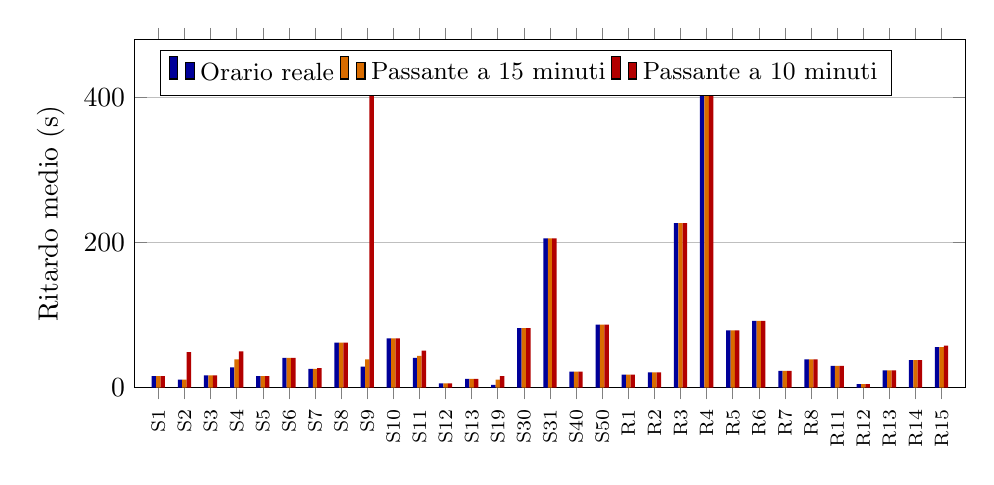
\begin{tikzpicture}
		\begin{axis}[ybar=0pt, bar width=1.6pt, width=\textwidth, height=6cm, symbolic x coords={S1,S2,S3,S4,S5,S6,S7,S8,S9,S10,S11,S12,S13,S19,S30,S31,S40,S50,R1,R2,R3,R4,R5,R6,R7,R8,R11,R12,R13,R14,R15}, xtick=data, x tick label style={rotate=90, font=\scriptsize}, ylabel={Ritardo medio (s)}, ymin=0, ymax=480, ymajorgrids, enlarge x limits=0.03, legend pos=north west, legend columns=3, legend style={font=\small}]
			\addplot[fill=blue!60!black, draw=none] coordinates {(S1,16) (S2,11) (S3,17) (S4,28) (S5,16) (S6,41) (S7,26) (S8,62) (S9,29) (S10,68) (S11,41) (S12,6) (S13,12) (S19,4) (S30,82) (S31,206) (S40,22) (S50,87) (R1,18) (R2,21) (R3,227) (R4,456) (R5,79) (R6,92) (R7,23) (R8,39) (R11,30) (R12,5) (R13,24) (R14,38) (R15,56)};
			\addplot[fill=orange!85!black, draw=none] coordinates {(S1,16) (S2,11) (S3,17) (S4,39) (S5,16) (S6,41) (S7,26) (S8,62) (S9,39) (S10,68) (S11,44) (S12,6) (S13,12) (S19,11) (S30,82) (S31,206) (S40,22) (S50,87) (R1,18) (R2,21) (R3,227) (R4,456) (R5,79) (R6,92) (R7,23) (R8,39) (R11,30) (R12,5) (R13,24) (R14,38) (R15,56)};
			\addplot[fill=red!70!black, draw=none] coordinates {(S1,16) (S2,49) (S3,17) (S4,50) (S5,16) (S6,41) (S7,27) (S8,62) (S9,405) (S10,68) (S11,51) (S12,6) (S13,12) (S19,16) (S30,82) (S31,206) (S40,22) (S50,87) (R1,18) (R2,21) (R3,227) (R4,456) (R5,79) (R6,92) (R7,23) (R8,39) (R11,30) (R12,5) (R13,24) (R14,38) (R15,58)};
			\legend{Orario reale, Passante a 15 minuti, Passante a 10 minuti}
		\end{axis}
	\end{tikzpicture}

	\medskip
	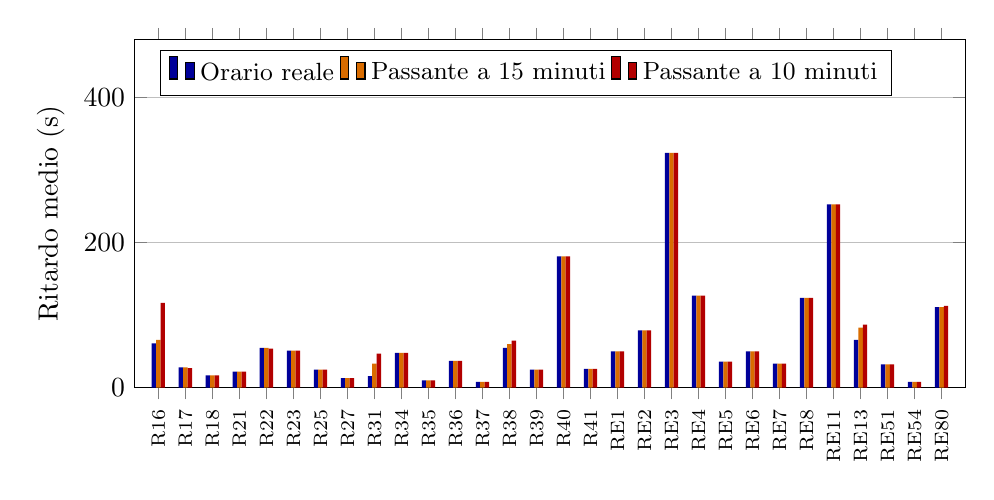
\begin{tikzpicture}
		\begin{axis}[ybar=0pt, bar width=1.6pt, width=\textwidth, height=6cm, symbolic x coords={R16,R17,R18,R21,R22,R23,R25,R27,R31,R34,R35,R36,R37,R38,R39,R40,R41,RE1,RE2,RE3,RE4,RE5,RE6,RE7,RE8,RE11,RE13,RE51,RE54,RE80}, xtick=data, x tick label style={rotate=90, font=\scriptsize}, ylabel={Ritardo medio (s)}, ymin=0, ymax=480, ymajorgrids, enlarge x limits=0.03, legend pos=north west, legend columns=3, legend style={font=\small}]
			\addplot[fill=blue!60!black, draw=none] coordinates {(R16,61) (R17,28) (R18,17) (R21,22) (R22,55) (R23,51) (R25,25) (R27,13) (R31,16) (R34,48) (R35,10) (R36,37) (R37,8) (R38,55) (R39,25) (R40,181) (R41,26) (RE1,50) (RE2,79) (RE3,324) (RE4,127) (RE5,36) (RE6,50) (RE7,33) (RE8,124) (RE11,253) (RE13,66) (RE51,32) (RE54,8) (RE80,111)};
			\addplot[fill=orange!85!black, draw=none] coordinates {(R16,66) (R17,28) (R18,17) (R21,22) (R22,55) (R23,51) (R25,25) (R27,13) (R31,33) (R34,48) (R35,10) (R36,37) (R37,8) (R38,60) (R39,25) (R40,181) (R41,26) (RE1,50) (RE2,79) (RE3,324) (RE4,127) (RE5,36) (RE6,50) (RE7,33) (RE8,124) (RE11,253) (RE13,83) (RE51,32) (RE54,8) (RE80,111)};
			\addplot[fill=red!70!black, draw=none] coordinates {(R16,117) (R17,27) (R18,17) (R21,22) (R22,54) (R23,51) (R25,25) (R27,13) (R31,47) (R34,48) (R35,10) (R36,37) (R37,8) (R38,65) (R39,25) (R40,181) (R41,26) (RE1,50) (RE2,79) (RE3,324) (RE4,127) (RE5,36) (RE6,50) (RE7,33) (RE8,124) (RE11,253) (RE13,87) (RE51,32) (RE54,8) (RE80,113)};
			\legend{Orario reale, Passante a 15 minuti, Passante a 10 minuti}
		\end{axis}
	\end{tikzpicture}
	\caption{Giorno feriale: ritardo medio per linea nell'orario reale e nello scenario del Passante a 15 e a 10 minuti.}
	\label{fig:linee-ritardo}
\end{figure}

\begin{figure}[H]
	\centering
	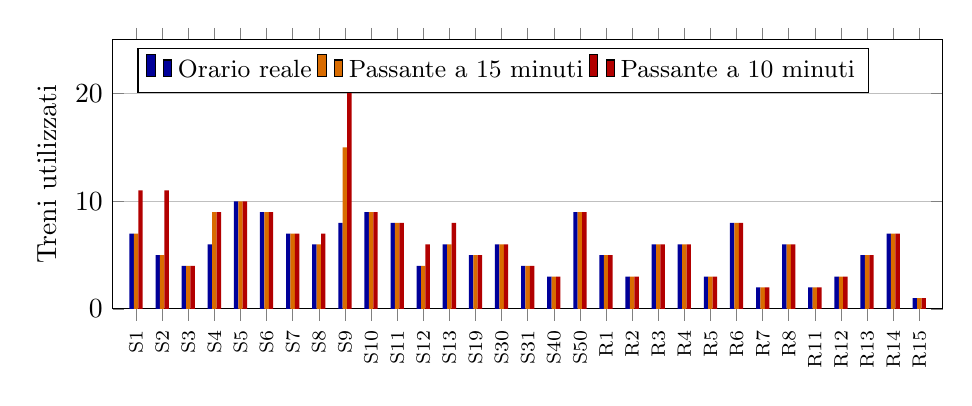
\begin{tikzpicture}
		\begin{axis}[ybar=0pt, bar width=1.6pt, width=\textwidth, height=5cm, symbolic x coords={S1,S2,S3,S4,S5,S6,S7,S8,S9,S10,S11,S12,S13,S19,S30,S31,S40,S50,R1,R2,R3,R4,R5,R6,R7,R8,R11,R12,R13,R14,R15}, xtick=data, x tick label style={rotate=90, font=\scriptsize}, ylabel={Treni utilizzati}, ymin=0, ymax=25, ymajorgrids, enlarge x limits=0.03, legend pos=north west, legend columns=3, legend style={font=\small}]
			\addplot[fill=blue!60!black, draw=none] coordinates {(S1,7) (S2,5) (S3,4) (S4,6) (S5,10) (S6,9) (S7,7) (S8,6) (S9,8) (S10,9) (S11,8) (S12,4) (S13,6) (S19,5) (S30,6) (S31,4) (S40,3) (S50,9) (R1,5) (R2,3) (R3,6) (R4,6) (R5,3) (R6,8) (R7,2) (R8,6) (R11,2) (R12,3) (R13,5) (R14,7) (R15,1)};
			\addplot[fill=orange!85!black, draw=none] coordinates {(S1,7) (S2,5) (S3,4) (S4,9) (S5,10) (S6,9) (S7,7) (S8,6) (S9,15) (S10,9) (S11,8) (S12,4) (S13,6) (S19,5) (S30,6) (S31,4) (S40,3) (S50,9) (R1,5) (R2,3) (R3,6) (R4,6) (R5,3) (R6,8) (R7,2) (R8,6) (R11,2) (R12,3) (R13,5) (R14,7) (R15,1)};
			\addplot[fill=red!70!black, draw=none] coordinates {(S1,11) (S2,11) (S3,4) (S4,9) (S5,10) (S6,9) (S7,7) (S8,7) (S9,23) (S10,9) (S11,8) (S12,6) (S13,8) (S19,5) (S30,6) (S31,4) (S40,3) (S50,9) (R1,5) (R2,3) (R3,6) (R4,6) (R5,3) (R6,8) (R7,2) (R8,6) (R11,2) (R12,3) (R13,5) (R14,7) (R15,1)};
			\legend{Orario reale, Passante a 15 minuti, Passante a 10 minuti}
		\end{axis}
	\end{tikzpicture}

	\medskip
	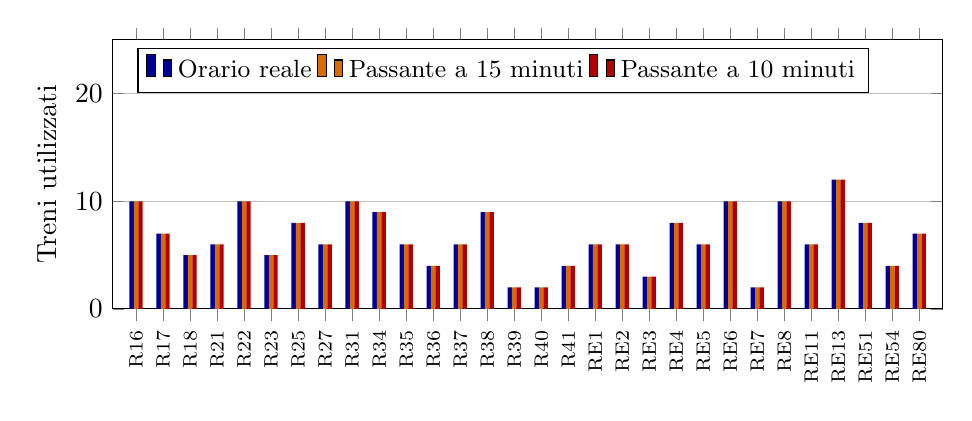
\begin{tikzpicture}
		\begin{axis}[ybar=0pt, bar width=1.6pt, width=\textwidth, height=5cm, symbolic x coords={R16,R17,R18,R21,R22,R23,R25,R27,R31,R34,R35,R36,R37,R38,R39,R40,R41,RE1,RE2,RE3,RE4,RE5,RE6,RE7,RE8,RE11,RE13,RE51,RE54,RE80}, xtick=data, x tick label style={rotate=90, font=\scriptsize}, ylabel={Treni utilizzati}, ymin=0, ymax=25, ymajorgrids, enlarge x limits=0.03, legend pos=north west, legend columns=3, legend style={font=\small}]
			\addplot[fill=blue!60!black, draw=none] coordinates {(R16,10) (R17,7) (R18,5) (R21,6) (R22,10) (R23,5) (R25,8) (R27,6) (R31,10) (R34,9) (R35,6) (R36,4) (R37,6) (R38,9) (R39,2) (R40,2) (R41,4) (RE1,6) (RE2,6) (RE3,3) (RE4,8) (RE5,6) (RE6,10) (RE7,2) (RE8,10) (RE11,6) (RE13,12) (RE51,8) (RE54,4) (RE80,7)};
			\addplot[fill=orange!85!black, draw=none] coordinates {(R16,10) (R17,7) (R18,5) (R21,6) (R22,10) (R23,5) (R25,8) (R27,6) (R31,10) (R34,9) (R35,6) (R36,4) (R37,6) (R38,9) (R39,2) (R40,2) (R41,4) (RE1,6) (RE2,6) (RE3,3) (RE4,8) (RE5,6) (RE6,10) (RE7,2) (RE8,10) (RE11,6) (RE13,12) (RE51,8) (RE54,4) (RE80,7)};
			\addplot[fill=red!70!black, draw=none] coordinates {(R16,10) (R17,7) (R18,5) (R21,6) (R22,10) (R23,5) (R25,8) (R27,6) (R31,10) (R34,9) (R35,6) (R36,4) (R37,6) (R38,9) (R39,2) (R40,2) (R41,4) (RE1,6) (RE2,6) (RE3,3) (RE4,8) (RE5,6) (RE6,10) (RE7,2) (RE8,10) (RE11,6) (RE13,12) (RE51,8) (RE54,4) (RE80,7)};
			\legend{Orario reale, Passante a 15 minuti, Passante a 10 minuti}
		\end{axis}
	\end{tikzpicture}
	\caption{Giorno feriale: treni utilizzati per linea nell'orario reale e nello scenario del Passante a 15 e a 10 minuti.}
	\label{fig:linee-treni}
\end{figure}

\subsubsection{Stazioni critiche e stazioni migliori}
Per ogni linea è stata calcolata, stazione per stazione, la media degli scostamenti dall'orario all'arrivo, con il segno: un valore positivo è un ritardo, uno negativo un anticipo. La \cref{tab:linee-stazioni} riporta per ogni linea la stazione con lo scostamento medio più alto, cioè il punto in cui la linea accumula ritardo, e quella con lo scostamento più basso. Sono considerate le stazioni con almeno cinque arrivi nella giornata; le linee R12 e RE7, con poche corse, non compaiono.

{\small
\begin{longtable}{@{}l>{\raggedright\arraybackslash}p{0.3\textwidth}r>{\raggedright\arraybackslash}p{0.3\textwidth}r@{}}
	\caption{Giorno feriale, orario reale: stazione con lo scostamento medio più alto e stazione con lo scostamento medio più basso, per linea. Valori in secondi; i negativi sono anticipi.}\label{tab:linee-stazioni}\\
	\toprule
	Linea & Stazione più critica & Scost. & Stazione migliore & Scost. \\
	\midrule
	\endfirsthead
	\toprule
	Linea & Stazione più critica & Scost. & Stazione migliore & Scost. \\
	\midrule
	\endhead
	S1 & Cesate & $+55$ & Milano Bovisa Politecnico & $-155$ \\
	S2 & Cesano Maderno & $+36$ & Meda & $-137$ \\
	S3 & Cesate & $+55$ & Milano Bovisa Politecnico & $-47$ \\
	S4 & Milano Domodossola & $+57$ & Paderno Dugnano & $-49$ \\
	S5 & Segrate & $+59$ & Treviglio & $-130$ \\
	S6 & Segrate & $+92$ & Treviglio & $-152$ \\
	S7 & Sesto S. Giovanni & $+56$ & Villasanta & $-54$ \\
	S8 & Sesto S. Giovanni & $+107$ & Lecco & $-57$ \\
	S9 & Ceriano Laghetto-Solaro & $+81$ & Milano Porta Garibaldi & $-458$ \\
	S10 & Melide & $+129$ & Chiasso & $-65$ \\
	S11 & Como Camerlata & $+79$ & Rho Fiera Milano & $-120$ \\
	S12 & Milano Porta Garibaldi Passante & $+15$ & Milano Bovisa Politecnico & $-187$ \\
	S13 & Certosa di Pavia & $+37$ & Milano Bovisa Politecnico & $-206$ \\
	S19 & Milano Romolo & $-21$ & Albairate & $-138$ \\
	S30 & Sangiano & $+113$ & Gallarate & $-91$ \\
	S31 & Brescia Violino & $+267$ & Iseo & $-40$ \\
	S40 & Balerna & $+48$ & Varese & $-113$ \\
	S50 & Melide & $+184$ & Malpensa Aeroporto T1 & $-40$ \\
	R1 & Rovato & $+26$ & Bergamo & $-102$ \\
	R2 & Verdello Dalmine & $+22$ & Treviglio & $-84$ \\
	R3 & Iseo & $+311$ & Edolo & $-196$ \\
	R4 & Treviglio & $+578$ & Brescia & $+162$ \\
	R5 & Cremona & $+170$ & Olmeneta & $+11$ \\
	R6 & Soresina & $+176$ & Milano Porta Garibaldi & $-95$ \\
	R7 & Calolziocorte Olginate & $+42$ & Lecco & $-64$ \\
	R8 & S. Zeno Folzano & $+101$ & Casalmaggiore & $-136$ \\
	R11 & Samolaco & $+52$ & Chiavenna & $-95$ \\
	R13 & Dervio & $+68$ & Colico & $-127$ \\
	R14 & Sesto S. Giovanni & $+79$ & Ponte S. Pietro & $-109$ \\
	R15 & Macherio Sovico & $+98$ & Carnate Usmate & $-58$ \\
	R16 & Milano Affori & $+97$ & Asso & $-67$ \\
	R17 & Como Borghi & $+76$ & Milano Bovisa Politecnico & $-58$ \\
	R18 & Como Camerlata & $+52$ & Molteno & $-94$ \\
	R21 & Porto Valtravaglia & $+49$ & Luino & $-131$ \\
	R22 & Malnate & $+112$ & Saronno & $-118$ \\
	R23 & Casorate Sempione & $+63$ & Arona & $-29$ \\
	R25 & Garbagna & $+45$ & Novara & $-111$ \\
	R27 & Galliate & $+22$ & Milano Cadorna & $-62$ \\
	R31 & Torreberetti & $+38$ & Milano Rogoredo & $-176$ \\
	R34 & Bressana Bottarone & $+133$ & Milano Porta Garibaldi & $-426$ \\
	R35 & Valmadonna & $+44$ & Pavia & $-258$ \\
	R36 & Nicorvo & $+83$ & Garlasco & $-151$ \\
	R37 & Ponte d'Adda & $+32$ & Corteolona & $-149$ \\
	R38 & Casalpusterlengo & $+100$ & Milano Greco Pirelli & $-99$ \\
	R39 & Acquanegra Cremonese & $+44$ & Cremona & $-98$ \\
	R40 & Gazzo Pieve S. Giacomo & $+206$ & Bozzolo & $+77$ \\
	R41 & Broni & $+64$ & Piacenza & $-41$ \\
	RE1 & Morosolo Casciago & $+119$ & Saronno & $-85$ \\
	RE2 & Bergamo & $+156$ & Milano Villapizzone & $-83$ \\
	RE3 & Brescia & $+409$ & Edolo & $-51$ \\
	RE4 & Sesto Calende & $+209$ & Rho Fiera Milano & $-55$ \\
	RE5 & Busto Arsizio & $+64$ & Rho Fiera Milano & $-153$ \\
	RE6 & Treviglio & $+84$ & Milano Centrale & $-124$ \\
	RE8 & Tresenda-Aprica-Teglio & $+270$ & Milano Rogoredo & $-127$ \\
	RE11 & Codogno & $+362$ & Milano Centrale & $+42$ \\
	RE13 & Alessandria & $+109$ & Milano Greco Pirelli & $-134$ \\
	RE51 & Milano Porta Garibaldi & $+79$ & Saronno & $-89$ \\
	RE54 & Malpensa Aeroporto T2 & $+17$ & Saronno & $-106$ \\
	RE80 & Lugano & $+263$ & Milano Centrale & $-42$ \\
	\bottomrule
\end{longtable}
}

Dalla tabella si ricavano quattro osservazioni:
\begin{itemize}
	\item le stazioni migliori sono quasi sempre capolinea o grandi nodi, con anticipi anche superiori a due minuti: il treno simulato viaggia sempre alla velocità massima e arriva prima dell'orario dove l'orario ha un margine prima dell'arrivo;
	\item sulle linee con il ritardo più alto il punto critico è un nodo condiviso con altre linee o una stazione di una tratta a binario unico: Treviglio per la R4, Brescia per la RE3, Codogno per la RE11, Iseo per la R3, Tresenda per la RE8;
	\item sulle linee R4, R5, R40 e RE11 anche la stazione migliore ha uno scostamento positivo: il ritardo riguarda l'intero percorso e non un solo punto;
	\item sulle linee S10 e S50 il punto critico è Melide, fra Lugano e Mendrisio, cioè il tratto in cui i treni delle due linee viaggiano accoppiati e il modello li simula come treni separati.
\end{itemize}
Negli scenari del Passante i punti critici si spostano. Con l'obiettivo di 15 minuti quello della S4 passa da Milano Domodossola a Cesano Maderno, con uno scostamento medio di 109 secondi, e quello della R16 a Milano Domodossola, con 116; per S9 e S2 resta quello dell'orario reale. Con l'obiettivo di 10 minuti il punto critico della S9 diventa Seveso Baruccana, sulla tratta a binario unico, con 827 secondi; per la S2 e la S4 è Cesano Maderno, con circa 185 secondi, e per la R16 Milano Domodossola, con 183.

\subsubsection{Potenziamento per linea}
La \cref{tab:linee-potenziamento} riporta per ogni linea la quota di corse completate e il ritardo medio nei tre casi del potenziamento. Il ritardo è misurato sulle sole fermate effettuate: dove le corse completate sono poche, un ritardo basso indica che sono arrivate soltanto le corse del mattino.

{\small
\begin{longtable}{@{}lrrrrrrr@{}}
	\caption{Potenziamento per linea, giorno feriale: corse completate e ritardo medio in secondi, per linea. La colonna \emph{reale} riporta il ritardo medio dell'orario reale.}\label{tab:linee-potenziamento}\\
	\toprule
	 & Reale & \multicolumn{2}{c}{Caso 1} & \multicolumn{2}{c}{Caso 2} & \multicolumn{2}{c}{Caso 3} \\
	Linea & ritardo & compl. & ritardo & compl. & ritardo & compl. & ritardo \\
	\midrule
	\endfirsthead
	\toprule
	 & Reale & \multicolumn{2}{c}{Caso 1} & \multicolumn{2}{c}{Caso 2} & \multicolumn{2}{c}{Caso 3} \\
	Linea & ritardo & compl. & ritardo & compl. & ritardo & compl. & ritardo \\
	\midrule
	\endhead
	S1 & 16 & 100\% & 17 & 77\% & 36 & 100\% & 17 \\
	S2 & 11 & 100\% & 23 & 88\% & 25 & 100\% & 23 \\
	S3 & 17 & 100\% & 17 & 83\% & 46 & 100\% & 17 \\
	S4 & 28 & 100\% & 34 & 82\% & 28 & 100\% & 34 \\
	S5 & 16 & 100\% & 24 & 75\% & 194 & 100\% & 26 \\
	S6 & 41 & 100\% & 52 & 73\% & 104 & 100\% & 52 \\
	S7 & 26 & 100\% & 996 & 94\% & 543 & 95\% & 610 \\
	S8 & 62 & 100\% & 4827 & 73\% & 1728 & 72\% & 1743 \\
	S9 & 29 & 100\% & 1849 & 85\% & 824 & 73\% & 830 \\
	S10 & 68 & 100\% & 176 & 100\% & 205 & 29\% & 478 \\
	S11 & 41 & 100\% & 2860 & 78\% & 1549 & 74\% & 1327 \\
	S12 & 6 & 100\% & 6 & 92\% & 34 & 100\% & 6 \\
	S13 & 12 & 100\% & 12 & 76\% & 18 & 100\% & 12 \\
	S19 & 4 & 100\% & 19 & 100\% & 16 & 100\% & 19 \\
	S30 & 82 & 100\% & 170 & 100\% & 154 & 100\% & 170 \\
	S31 & 206 & 100\% & 205 & 100\% & 205 & 100\% & 205 \\
	S40 & 22 & 100\% & 108 & 100\% & 116 & 46\% & 142 \\
	S50 & 87 & 100\% & 167 & 100\% & 156 & 29\% & 145 \\
	R1 & 18 & 100\% & 54 & 100\% & 90 & 100\% & 54 \\
	R2 & 21 & 100\% & 22 & 100\% & 153 & 100\% & 22 \\
	R3 & 227 & 100\% & 171 & 100\% & 171 & 100\% & 171 \\
	R4 & 456 & 100\% & 1223 & 91\% & 894 & 91\% & 882 \\
	R5 & 79 & 25\% & 396 & 25\% & 313 & 25\% & 396 \\
	R6 & 92 & 32\% & 169 & 32\% & 197 & 32\% & 175 \\
	R7 & 23 & 100\% & 44 & 100\% & 44 & 100\% & 44 \\
	R8 & 39 & 100\% & 86 & 100\% & 83 & 100\% & 86 \\
	R11 & 30 & 100\% & 876 & 100\% & 872 & 90\% & 893 \\
	R12 & 5 & 100\% & 5 & 100\% & 5 & 100\% & 5 \\
	R13 & 24 & 95\% & 965 & 100\% & 627 & 79\% & 316 \\
	R14 & 38 & 100\% & 2785 & 83\% & 1151 & 80\% & 1694 \\
	R15 & 56 & 100\% & 102 & 100\% & 86 & 100\% & 86 \\
	R16 & 61 & 100\% & 260 & 96\% & 333 & 100\% & 260 \\
	R17 & 28 & 100\% & 28 & 100\% & 135 & 100\% & 28 \\
	R18 & 17 & 100\% & 85 & 100\% & 62 & 100\% & 81 \\
	R21 & 22 & 100\% & 71 & 100\% & 157 & 100\% & 71 \\
	R22 & 55 & 100\% & 82 & 100\% & 2768 & 100\% & 82 \\
	R23 & 51 & 100\% & 91 & 76\% & 216 & 100\% & 83 \\
	R25 & 25 & 100\% & 292 & 100\% & 292 & 100\% & 292 \\
	R27 & 13 & 100\% & 24 & 100\% & 41 & 100\% & 24 \\
	R31 & 16 & 100\% & 131 & 100\% & 155 & 100\% & 158 \\
	R34 & 48 & 100\% & 50 & 100\% & 50 & 100\% & 50 \\
	R35 & 10 & 100\% & 27 & 100\% & 27 & 100\% & 27 \\
	R36 & 37 & 100\% & 1584 & 100\% & 1584 & 100\% & 1584 \\
	R37 & 8 & 59\% & 799 & 45\% & 505 & 59\% & 799 \\
	R38 & 55 & 70\% & 59 & 55\% & 139 & 70\% & 60 \\
	R39 & 25 & 67\% & 28 & 67\% & 28 & 67\% & 28 \\
	R40 & 181 & 38\% & 38 & 38\% & 38 & 38\% & 38 \\
	R41 & 26 & 100\% & 26 & 100\% & 26 & 100\% & 26 \\
	RE1 & 50 & 100\% & 48 & 100\% & 3177 & 100\% & 48 \\
	RE2 & 79 & 100\% & 51 & 91\% & 312 & 100\% & 50 \\
	RE3 & 324 & 100\% & 288 & 100\% & 288 & 100\% & 288 \\
	RE4 & 127 & 100\% & 141 & 99\% & 165 & 100\% & 139 \\
	RE5 & 36 & 100\% & 149 & 89\% & 479 & 100\% & 162 \\
	RE6 & 50 & 100\% & 56 & 100\% & 82 & 100\% & 58 \\
	RE7 & 33 & 100\% & 35 & 100\% & 179 & 100\% & 35 \\
	RE8 & 124 & 75\% & 4023 & 84\% & 4836 & 70\% & 3473 \\
	RE11 & 253 & 30\% & 219 & 30\% & 272 & 30\% & 219 \\
	RE13 & 66 & 100\% & 84 & 100\% & 66 & 97\% & 71 \\
	RE51 & 32 & 100\% & 32 & 78\% & 46 & 100\% & 32 \\
	RE54 & 8 & 100\% & 8 & 100\% & 260 & 100\% & 8 \\
	RE80 & 111 & 100\% & 425 & 99\% & 305 & 34\% & 619 \\
	\bottomrule
\end{longtable}
}
